\documentclass[aspectratio=169,10pt]{beamer}

% ── Font: Carlito (metric-compatible Calibri replacement) ─────────────────
\usepackage[sfdefault,lf]{carlito}
\usepackage[T1]{fontenc}

% ── Theme ──────────────────────────────────────────────────────────────────
\usetheme{default}
\setbeamertemplate{navigation symbols}{}
\setbeamertemplate{footline}{%
  \hfill\small\insertframenumber\,/\,\inserttotalframenumber\hspace{6pt}\vspace{4pt}%
}
\setbeamertemplate{itemize item}{\color{mainBlue}\textbullet}
\setbeamertemplate{itemize subitem}{\color{mainBlue!60}$\circ$}

% ── Colours ────────────────────────────────────────────────────────────────
\definecolor{mainBlue}{RGB}{23,54,115}
\definecolor{accentGold}{RGB}{196,158,84}
\definecolor{lightBg}{RGB}{245,247,252}

\setbeamercolor{frametitle}{bg=mainBlue,fg=white}
\setbeamercolor{structure}{fg=mainBlue}
\setbeamercolor{normal text}{fg=black!85}
\setbeamercolor{block title}{bg=mainBlue,fg=white}
\setbeamercolor{block body}{bg=lightBg,fg=black!85}
\setbeamercolor{alerted text}{fg=accentGold!80!black}

\setbeamerfont{frametitle}{size=\large,series=\bfseries}

% ── Packages ───────────────────────────────────────────────────────────────
\usepackage{graphicx}
\usepackage{booktabs}
\usepackage{xcolor}
\usepackage{amsmath}
\usepackage{tikz}

\graphicspath{
  {/Users/he/jcSOLID/deliverables/paper/figures/}
  {/Users/he/jcSOLID/deliverables/slides/}
}

% ── Metadata ───────────────────────────────────────────────────────────────
\title{Diff-Eval}
\subtitle{An AI-Driven Agentic Workflow for Code Quality Evaluation}
\author{Jiahe (Jay) Chen}
\institute{Duke Kunshan University \quad|\quad Mentor: Prof.\ Jiacheng Shen}
\date{March 2026}

% ============================================================
\begin{document}

% ── SLIDE 1 · Title ─────────────────────────────────────────────────────────
{
\setbeamertemplate{footline}{}
\begin{frame}
  \vspace{0.3cm}
  \begin{columns}[c]
    \column{0.73\textwidth}
      {\color{mainBlue}\LARGE\bfseries Diff-Eval\par}
      \vspace{0.15cm}
      {\color{mainBlue!70}\large An AI-Driven Agentic Workflow for Code Quality Evaluation\par}
      \vspace{0.4cm}
      
\begin{tikzpicture}
        \draw[mainBlue,line width=1.2pt] (0,0) -- (8,0);
      \end{tikzpicture}
      \vspace{0.25cm}
      {\normalsize\textbf{Jiahe~(Jay)~Chen}\par}
      {\small Computation and Design (Computer Science)\par}
      {\small Duke Kunshan University\par}
      \vspace{0.12cm}
      {\small Mentor: Prof.\ Jiacheng Shen, Assistant Professor of ECE\par}
      \vspace{0.12cm}
      {\small March 2026\par}
    \column{0.23\textwidth}
      \centering
      \includegraphics[width=\textwidth]{DKU Logo_Vertical _2_.png}
  \end{columns}
\end{frame}
}

% ── SLIDE 2 · Introduction ───────────────────────────────────────────────────
\begin{frame}{Introduction: The Problem}
  \vspace{0.3cm}
  \begin{block}{}
    \centering\normalsize\itshape
    ``Code quality is a critical concern in software engineering, directly\\
    affecting system stability, maintainability, and development efficiency.''
  \end{block}
  \vspace{0.5cm}
  \begin{columns}[T]
    \column{0.48\textwidth}
      \textbf{What Static Analyzers Do}
      \begin{itemize}\small
        \item Rule-based pattern matching (SonarQube, Checkstyle, PMD)
        \item Fast and reliable for syntactic/structural issues
      \end{itemize}
    \column{0.48\textwidth}
      \textbf{Where They Fall Short}
      \begin{itemize}\small
        \item Cannot understand \emph{architectural intent}
        \item Fail to detect \textbf{design-level} violations (e.g.\ SOLID)
        \item Require understanding \emph{why} code is structured the way it is
      \end{itemize}
  \end{columns}
\end{frame}

% ── SLIDE 3 · Background – SOLID ────────────────────────────────────────────
\begin{frame}{Background: SOLID Principles}
  \vspace{0.2cm}
  \begin{columns}[T]
    \column{0.45\textwidth}
      \textbf{SOLID (R.\,C.\ Martin, 2000)}
      \vspace{0.2cm}
      \begin{tabular}{@{}lp{0.75\linewidth}@{}}
        \toprule
        \textbf{S} & Single Responsibility — one reason to change \\[3pt]
        \textbf{O} & Open / Closed — open for extension, closed for modification \\[3pt]
        \textbf{L} & Liskov Substitution — subtypes replaceable for base types \\[3pt]
        \textbf{I} & Interface Segregation — no forced unused dependencies \\[3pt]
        \textbf{D} & Dependency Inversion — depend on abstractions, not concretions \\
        \bottomrule
      \end{tabular}

    \column{0.50\textwidth}
      \textbf{Why SOLID Matters}
      \begin{itemize}\small
        \item Violations produce \textbf{rigid, fragile, tightly coupled} code
        \item Resist future modification and raise maintenance costs
        \item Hard to detect automatically — requires understanding \emph{intent}, not just syntax
      \end{itemize}
      \vspace{0.3cm}
      \begin{block}{The Detection Challenge}
        \small Static analyzers catch \emph{syntax}. SOLID violations are \emph{structural} and \emph{semantic} — they require reasoning about architectural design intent.
      \end{block}
  \end{columns}
\end{frame}

% ── SLIDE 4 · Background – LLMs & Benchmark ─────────────────────────────────
\begin{frame}{Background: LLM-Based Detection \& Benchmark Dataset}
  \begin{columns}[T]
    \column{0.46\textwidth}
      \textbf{Pehlivan et al.\ (2025)}
      \begin{itemize}\small
        \item First systematic study: 4 models, 4 prompt strategies
        \item Best: \texttt{example} (few-shot) strategy
        \item GPT-4o-mini peaks at \textbf{69.2\%}; open-source $<$25\%
        \item DIP essentially unsolved: F1 = 0–10.8
        \item Qwen family top open-source performer $\Rightarrow$ motivates model choice
      \end{itemize}
      \vspace{0.08cm}
      \begin{block}{Benchmark Dataset}
        \begin{itemize}\small
          \item 240 examples, 48 per SOLID principle
          \item 4 languages: Python, Java, Kotlin, C\#
          \item Easy (33 LOC) / Moderate (140 LOC) / Hard (306 LOC)
        \end{itemize}
      \end{block}

    \column{0.50\textwidth}
      \centering
      
\includegraphics[width=\textwidth,height=0.36\textheight,keepaspectratio]{solid_violations_f1_by_model.png}
      \vspace{0.06cm}
      
\includegraphics[width=\textwidth,height=0.36\textheight,keepaspectratio]{solid_violations_accuracy_by_level.png}
  \end{columns}
\end{frame}

% ── SLIDE 5 · Background – Agentic & Baselines ──────────────────────────────
\begin{frame}{Background: Agentic Workflows \& Baselines}
  \begin{columns}[T]
    \column{0.51\textwidth}
      \textbf{Melo et al.\ (2025) — Test Smell Detection}
      \begin{itemize}\small
        \item Applied agentic workflows to code quality with small models (3B–14B)
        \item Detector–Evaluator feedback loop outperforms single-pass
        \item Phi-4-14B (4 agents) within 5\% of single-agent GPT-4o-mini
      \end{itemize}
      \vspace{0.1cm}
      
\includegraphics[width=\textwidth,height=0.38\textheight,keepaspectratio]{test_smell_agent.png}

    \column{0.45\textwidth}
      \textbf{Our Baselines — both use Qwen3.5 9B}
      \vspace{0.15cm}
      \begin{block}{Single Agent}
        \begin{itemize}\small
          \item Replicates Pehlivan \texttt{example} strategy
          \item Code in $\to$ violated principle out
        \end{itemize}
      \end{block}
      \vspace{0.15cm}
      \begin{block}{Two-Agent (Detector + Evaluator)}
        \begin{itemize}\small
          \item Agent 1 detects with reasoning
          \item Agent 2 critiques \& refines (up to 3 rounds)
          \item Adopts Melo et al.\ pattern
        \end{itemize}
      \end{block}
      \vspace{0.2cm}
      \begin{itemize}\small
        \item Same model across all three workflows
        \item Differences $\Rightarrow$ \textbf{workflow design}, not model scale
      \end{itemize}
  \end{columns}
\end{frame}

% ── SLIDE 6 · Our Design ────────────────────────────────────────────────────
\begin{frame}{Diff Eval: System Design}
  % ── Architecture image — upper half ──────────────────────────────────────
  \begin{center}
    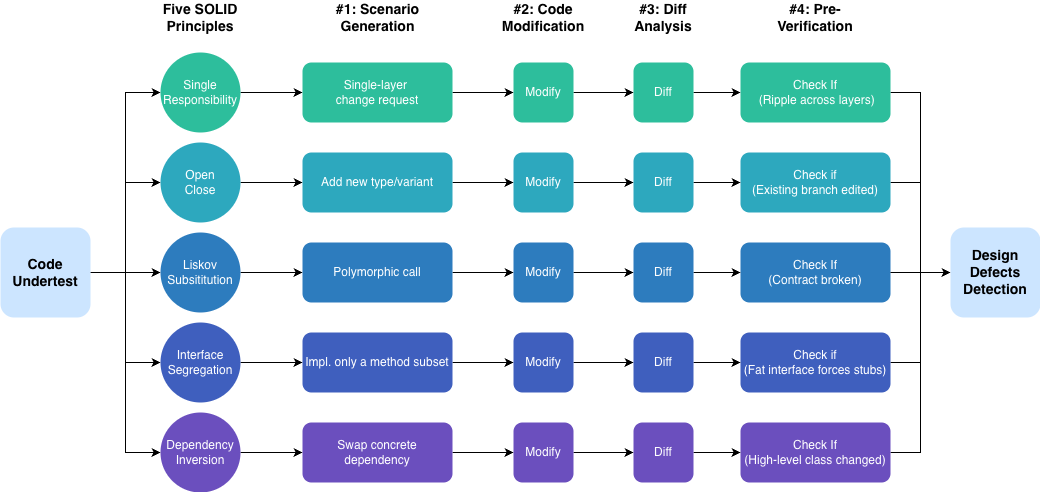
\includegraphics[width=\textwidth,height=0.55\textheight,keepaspectratio]{architecture_updated.png}
  \end{center}
  {\small\color{mainBlue}\textbf{Core Design:}
   simulates real software development scenarios by modifying the code proactively to test the extendability}

  \begin{columns}[T]
    \column{0.19\textwidth}
      \centering
      {\footnotesize\textbf{\color{mainBlue}Scenario Gen.}}\\[0pt]
      {\footnotesize Principle-specific extension task engineered to trigger violation}
    \column{0.19\textwidth}
      \centering
      {\footnotesize\textbf{\color{mainBlue}Code Modification}}\\[0pt]
      {\footnotesize LLM implements the scenario on the original code}
    \column{0.19\textwidth}
      \centering
      {\footnotesize\textbf{\color{mainBlue}Diff Analysis}}\\[0pt]
      {\footnotesize Unified diff computed via Python \texttt{difflib}}
    \column{0.19\textwidth}
      \centering
      {\footnotesize\textbf{\color{mainBlue}Pre-Verification}}\\[0pt]
      {\footnotesize Diff pattern matched to principle's violation signal}
    \column{0.19\textwidth}
      \centering
      {\footnotesize\textbf{\color{mainBlue}Unified Ranking}}\\[0pt]
      {\footnotesize Aggregates 5 verdicts $\to$ Top-N ranked output}
  \end{columns}
\end{frame}

% ── SLIDE 7 · Results – Overall ─────────────────────────────────────────────
\begin{frame}{Results: Overall Performance}
  \begin{columns}[T]
    \column{0.50\textwidth}
      \centering
      
\includegraphics[width=\textwidth,height=0.65\textheight,keepaspectratio]{paper_fig_overall.png}

    \column{0.46\textwidth}
      \vspace{0.2cm}
      {\small
      \begin{tabular}{@{}lccc@{}}
        \toprule
        \textbf{Method} & \textbf{Acc.} & \textbf{MRR@2} & \textbf{F1} \\
        \midrule
        Single Agent       & 70.00\% & 0.638 & 0.699 \\
        Two-Agent          & 55.83\% & 0.490 & 0.576 \\
        \textbf{Diff Eval} & \textbf{87.92\%} & \textbf{0.792} & \textbf{0.888} \\
        \bottomrule
      \end{tabular}}
      \vspace{0.3cm}
      \begin{itemize}\small
        \item \textbf{+17.9 pp} over Single Agent
        \item \textbf{+32.1 pp} over Two-Agent
        \item Macro-F1 0.888 — balanced across all five principles
        \item Two-Agent \emph{underperforms} SA:\\
              debate without better evidence degrades accuracy
        \item \textit{Metric}: Top-2 Accuracy — ground-truth violation
              appears in model's top-2 predictions
      \end{itemize}
  \end{columns}
\end{frame}

% ── SLIDE 8 · Results – By Violation & Difficulty ───────────────────────────
\begin{frame}{Results: By Violation Type \& Difficulty Level}
  \begin{columns}[T]
    \column{0.48\textwidth}
      \centering
      {\small\textbf{By SOLID Principle}}\\[4pt]
      
\includegraphics[width=\textwidth,height=0.43\textheight,keepaspectratio]{paper_fig_violation.png}
      \vspace{0.1cm}
      \begin{itemize}\footnotesize
        \item \textbf{DIP}: 20.83\% (SA) $\to$ \textbf{91.67\%} (Diff Eval)\\
              Tight coupling invisible statically; concrete in diffs
        \item \textbf{ISP}: 83.33\% $\to$ \textbf{97.92\%}
        \item \textbf{OCP}: SA leads (97.92\% vs.\ 72.92\%)\\
              Surface \texttt{if-else} — direct inspection wins
      \end{itemize}

    \column{0.48\textwidth}
      \centering
      {\small\textbf{By Difficulty Level}}\\[4pt]
      
\includegraphics[width=\textwidth,height=0.43\textheight,keepaspectratio]{paper_fig_difficulty.png}
      \vspace{0.1cm}
      \begin{itemize}\footnotesize
        \item Diff Eval leads at \textbf{every} difficulty level
        \item Easy$\to$Hard drop: \textbf{12.5 pp} vs.\ 11.25 pp (SA) / 15 pp (TA)
        \item Hard: \textbf{80.00\%} vs.\ 63.75\% (SA) / 45.00\% (TA)
        \item Pre-Verification passes only the compact diff\\
              $\Rightarrow$ insulates ranking from long-code noise
      \end{itemize}
  \end{columns}
\end{frame}

% ── SLIDE 9 · Results – Cloud Comparison ────────────────────────────────────
\begin{frame}{Results: Comparison with Full-Size Cloud LLM}
  \vspace{0.15cm}
  \begin{center}
    \small
    \begin{tabular}{@{}lcc@{}}
      \toprule
      \textbf{System} & \textbf{Top-2 Accuracy} & \textbf{MRR@2} \\
      \midrule
      Qwen3.5 9B — Single Agent \footnotesize(local)       & 70.00\% & 0.638 \\
      \textbf{Qwen3.5 9B — Diff Eval} \footnotesize(local) & \textbf{87.92\%} & \textbf{0.792} \\
      \midrule
      Qwen3.5 Plus — Single Agent \footnotesize(cloud)     & 95.83\% & 0.858 \\
      \bottomrule
    \end{tabular}
  \end{center}
  \vspace{0.25cm}
  \begin{columns}[T]
    \column{0.50\textwidth}
      \begin{block}{Key Finding}
        \begin{itemize}\small
          \item Plain 9B baseline lags cloud by \textbf{25.83 pp}
          \item Diff Eval recovers \textbf{17.92 pp} through workflow design alone
          \item Closes \textbf{$\sim$70\%} of gap — no increase in model size
          \item \textbf{Zero data egress}
        \end{itemize}
      \end{block}
    \column{0.46\textwidth}
      \textbf{Why it matters}
      \begin{itemize}\small
        \item Regulated code cannot leave the premises
        \item Consumer hardware: RTX 4060 8GB, i5-12400F
        \item On DIP specifically: Diff Eval \textbf{matches} Qwen3.5 Plus (91.67\%)
        \item Entire pipeline is \textbf{observable}: every diff, verdict, and ranking rationale is logged
      \end{itemize}
  \end{columns}
\end{frame}

% ── SLIDE 10 · Discussion ────────────────────────────────────────────────────
\begin{frame}{Discussion}
  \begin{columns}[T]
    \column{0.50\textwidth}
      \textbf{Error Analysis — SRP Over-prediction}
      \begin{itemize}\small
        \item 29 total errors; \textbf{19} are SRP over-prediction
        \item OCP$\to$SRP (11), LSP$\to$SRP (5), DIP$\to$SRP (3)
        \item Responsibility-mixing symptoms appear across violation types\\
              $\Rightarrow$ conceptual overlap inherent in SOLID taxonomy
      \end{itemize}
      \vspace{0.06cm}
      \centering
      
\includegraphics[width=0.95\textwidth,height=0.42\textheight,keepaspectratio]{paper_fig_confusion.png}

    \column{0.46\textwidth}
      \textbf{Why Diff Eval Works}
      \begin{itemize}\small
        \item Abstract judgment $\to$ \textbf{concrete evidence}
        \item DIP \& ISP: invisible statically, concrete in diffs
        \item Pre-Verification compresses context for robustness
      \end{itemize}
      \vspace{0.15cm}
      \textbf{Limitations}
      \begin{itemize}\small
        \item \textbf{OCP} (72.92\%): SRP scenario absorbs OCP signals
        \item \textbf{Runtime}: 20 calls/example (151.6 s) vs.\ 1 call (2.1 s)
        \item \textbf{Dataset}: 240 examples only
      \end{itemize}
      \vspace{0.15cm}
      \textbf{Observability \& Privacy}
      \begin{itemize}\small
        \item Every artifact persisted and inspectable
        \item Transparent reasoning — not a black box
        \item Compliant: EU AI Act, Katakri 2020
      \end{itemize}
  \end{columns}
\end{frame}

% ── SLIDE 11 · Conclusion ───────────────────────────────────────────────────
{
\setbeamertemplate{footline}{}
\begin{frame}{Conclusion}
  \begin{columns}[T]
    \column{0.68\textwidth}
      \begin{block}{\centering Small LLM + Agentic Workflow $\approx$ Full-Size LLM}
        \centering\small in the code quality evaluation scenario
      \end{block}
      \vspace{0.1cm}
      \textbf{Results}
      \begin{itemize}\small
        \item \textbf{87.92\% accuracy} on SOLID detection using a local 9B model
        \item Closes \textbf{$\sim$70\%} of gap to Qwen3.5 Plus (95.83\%) through workflow design alone
        \item Consumer hardware, \textbf{zero data egress}
        \item +17.9 pp over single-agent; balanced across all five principles
        \item Design quality best revealed by \textbf{behavioral observation}\\
              (what happens when you extend the code), not static judgment
      \end{itemize}
      \vspace{0.1cm}
      \textbf{Future Work}
      \begin{enumerate}\small
        \item Hybrid: best method per principle
        \item Improved OCP scenario generation
        \item Larger-scale evaluation on real codebases
      \end{enumerate}

    \column{0.28\textwidth}
      \centering
      \vspace{0.2cm}
      \includegraphics[width=0.82\textwidth]{DKU Logo_Vertical _2_.png}
      \vspace{0.3cm}
      {\small\color{mainBlue}
        \textbf{Jiahe (Jay) Chen}\\[4pt]
        Mentor: Prof.\ Jiacheng Shen\\[2pt]
        Duke Kunshan University\\[2pt]
        Class of 2026
      }
  \end{columns}
\end{frame}
}

% ── SLIDE 12 · References ───────────────────────────────────────────────────
{
\setbeamertemplate{footline}{}
\begin{frame}{References}
  \begin{columns}[T]
    \column{0.49\textwidth}
      {\footnotesize
      \begin{enumerate}
        \item R.\,C.\ Martin, ``Design Principles and Design Patterns,'' 2000.
        \item R.\,C.\ Martin, \textit{Clean Architecture}, Prentice Hall, 2017.
        \item Pehlivan et al., ``Evaluating LLMs for SOLID Violation Detection,''
              \textit{arXiv}, 2025.
        \item Melo et al., ``Agentic LLM Workflows for Test Smell Detection,''
              \textit{arXiv}, 2025.
        \item Sharma et al., ``Designite: A Software Design Quality Assessment Tool,''
              \textit{ICSE}, 2018.
        \item Palomba et al., ``Detecting Bad Smells Using Change History,''
              \textit{ASE}, 2015.
      \end{enumerate}
      }
    \column{0.49\textwidth}
      {\footnotesize
      \begin{enumerate}\setcounter{enumi}{6}
        \item Wang et al., ``A Survey on LLM-Based Autonomous Agents,''
              \textit{Front.\ Comput.\ Sci.}, 2024.
        \item Yao et al., ``ReAct: Synergizing Reasoning and Acting in LLMs,''
              \textit{ICLR}, 2023.
        \item LangChain Inc., \textit{LangGraph}, 2024.
        \item Ollama, \textit{Local LLM Inference Framework}, 2024.
        \item Qwen Team, ``Qwen2.5 Technical Report,'' \textit{arXiv}, 2025.
        \item European Parliament, \textit{EU AI Act}, 2024.
        \item Al-Omar et al., ``On the Relationship Between Code Smells and SOLID,''
              \textit{JSS}, 2023.
      \end{enumerate}
      }
  \end{columns}
\end{frame}
}

\end{document}
